\section{Background estimation}\label{chap5:backgrounds}

The main background processes affecting the analysis signature, non-resonant WW production and top quark processes, are estimated using data. Backgrounds arising from an experimental misidentification of the objects, such as W+jets (also called ``Fake''), are estimated using data as well. The other minor backgrounds are generally estimated directly from simulation as described in the following subsections.

\subsection{WW background}

The quark-induced WW background is simulated with NLO accuracy in perturbative QCD, and the transverse momentum of the diboson system is reweighted to match the NNLO+NNLL accuracy from theoretical calculations~\cite{Meade:2014fca,Jaiswal:2014yba}. However, given the large uncertainties on the jet multiplicity distribution associated to this process, the normalization of this background is measured from data separately for the 0 and 1 jet categories. The normalization k-factors are extracted directly from the fit together with the signal strengths, leaving the WW normalization free to float separately in the two jet multiplicity categories. An orthogonal control region for the WW background normalization estimation is not needed in this case, owing to the different $m_{\ell\ell}$-$\mt$ shape for signal and background.

The gluon-induced WW production is sub-dominant with respect to the quark-induced production, and its shape and normalization is fully taken from simulation, scaling the cross section to the theoretical prediction with NLO accuracy~\cite{Caola:2015rqy}.

\subsection{Top quark background}

As explained in Sec.~\ref{chap5:analysis_strategy}, the production of top quark pairs represents one of the dominant backgrounds in this analysis given its large cross section and a similar final state compared to the signal. A b-jet veto, based on the \emph{cMVAv2} b tagging algorithm, is used to suppress this background and a reweighting procedure is applied on top of the simulated events to correct for different b tagging efficiency in data and simulation.

The top quark background normalization is measured using data, defining a b-jets enriched control region by inverting the b-jet veto. More precisely, the b-jets enriched control region for the 0-jet category is defined with the same WW baseline selection but requiring at least one jet with $20<\pt<30$\GeV to be identified as a b jet and no other jets with $\pt > 30$\GeV. For the 1-jet category, the b-jets enriched region is defined requiring exactly one jet with $\pt>30$\GeV identified as a b-jet.
To reduce other backgrounds in these two regions, the dilepton mass has to be greater than 50\GeV. Distributions of the \mll and \mt variables in the b-jets enriched control regions after applying the data driven estimation are shown in Figure~\ref{fig:TopCtrl}, for the 0 and 1 jet categories separately.

The top quark background normalization is constrained during the fit procedure separately in the two jet categories, by means of the control regions defined above, which are treated in the fit as two additional categories. 

\begin{figure}[htbp]
\centering
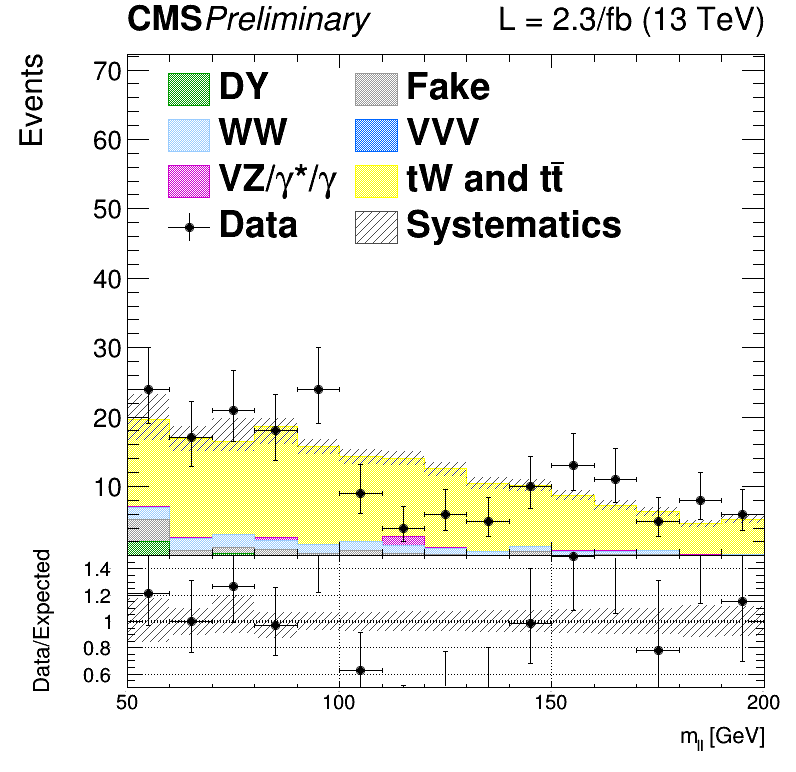
\includegraphics[width=0.45\textwidth]{images/13TeV/cratio_hww2l2v_13TeV_top_of0j_mll.png}
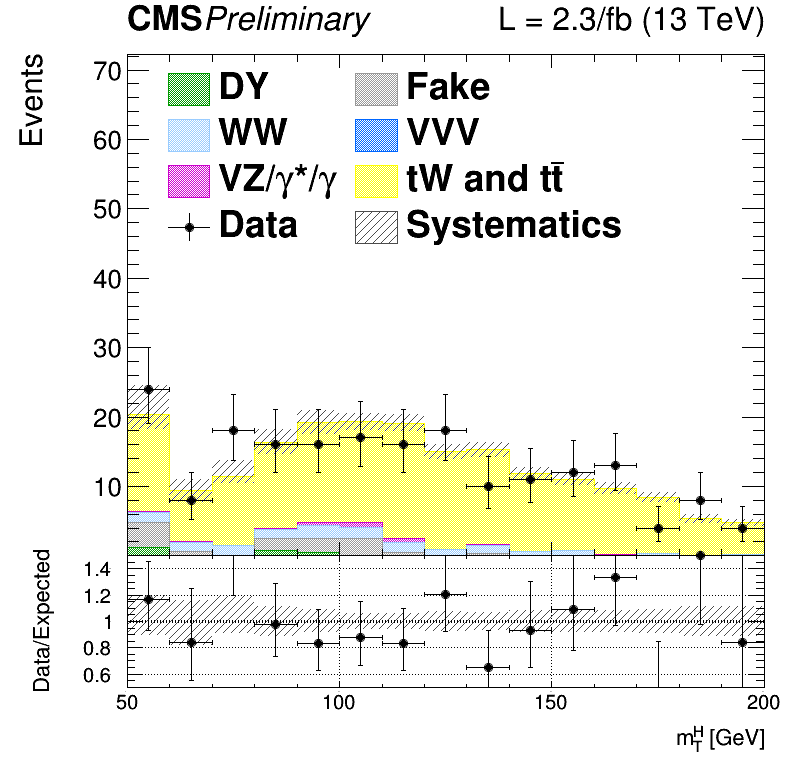
\includegraphics[width=0.45\textwidth]{images/13TeV/cratio_hww2l2v_13TeV_top_of0j_mth.png}
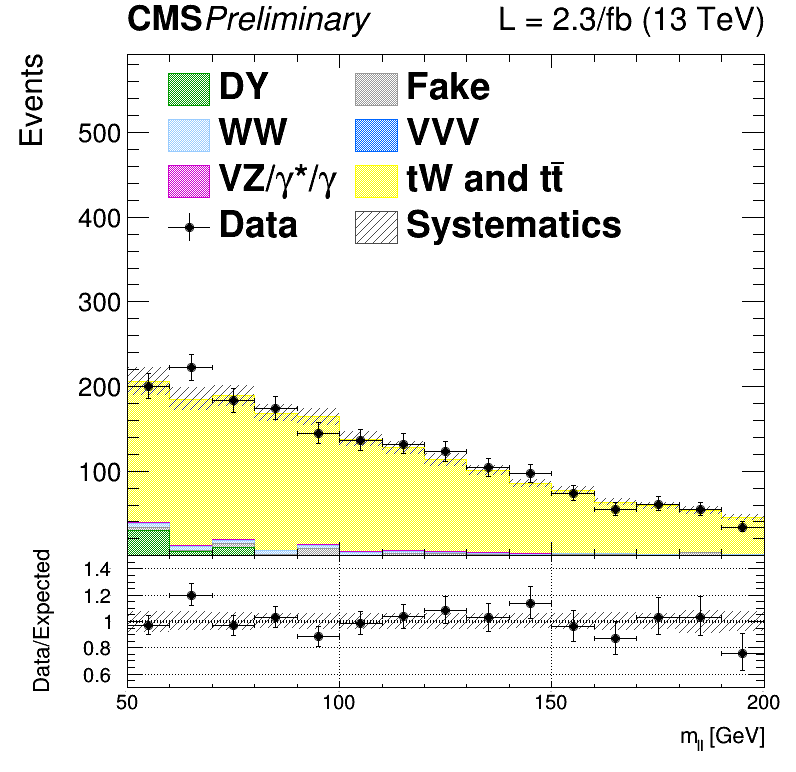
\includegraphics[width=0.45\textwidth]{images/13TeV/cratio_hww2l2v_13TeV_top_of1j_mll.png}
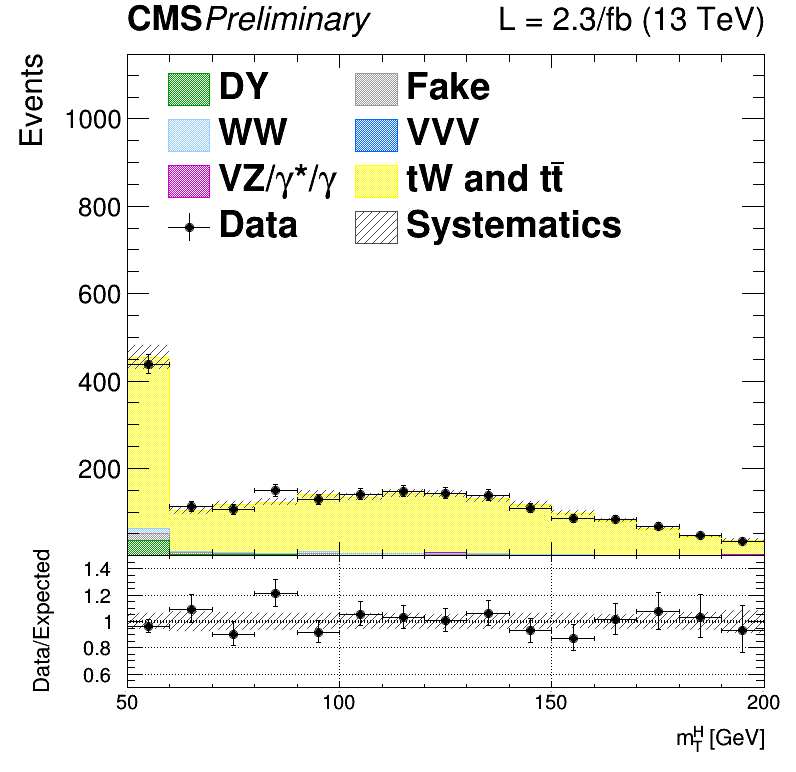
\includegraphics[width=0.45\textwidth]{images/13TeV/cratio_hww2l2v_13TeV_top_of1j_mth.png}
\caption{
Distributions of \mll (left) and \mt (right) for events with 0 jet (top) and 1 jet (bottom) 
in top enriched phase space.
Scale factors estimated from data are applied. The first (last) bin includes underflows (overflows).
}
\label{fig:TopCtrl}
\end{figure}

\subsection{Jet-induced (or Fake) background}

One of the primary source belonging to this category arises from the misidentification of leptons in W+jets processes in the 0 jet category. Also, semileptonic \ttbar decays contribute especially for higher jet multiplicities. Multijet production and hadronic \ttbar decays are also taken into account, but have a much smaller contribution.

This background is fully estimated using data, with the technique described in Sec.~\ref{sec:wjetsbkg}. To check the agreement of the background estimated in this way with data, a control sample enriched in jet-induced events is defined. The events in the control sample are selected applying the WW baseline requirements but requesting an e$\mu$ pair with same charge, which significantly suppresses the WW and \ttbar processes. The \mll distributions in this control region for the 0 and 1 jet categories are shown in Fig.~\ref{fig:13TeVsamesign}. From the crosscheck in this control region, a global normalization factor of 0.8 is derived and applied to the jet-induced background.

\begin{figure}[!h]
\centering
    \subfigure[0 jet]{
    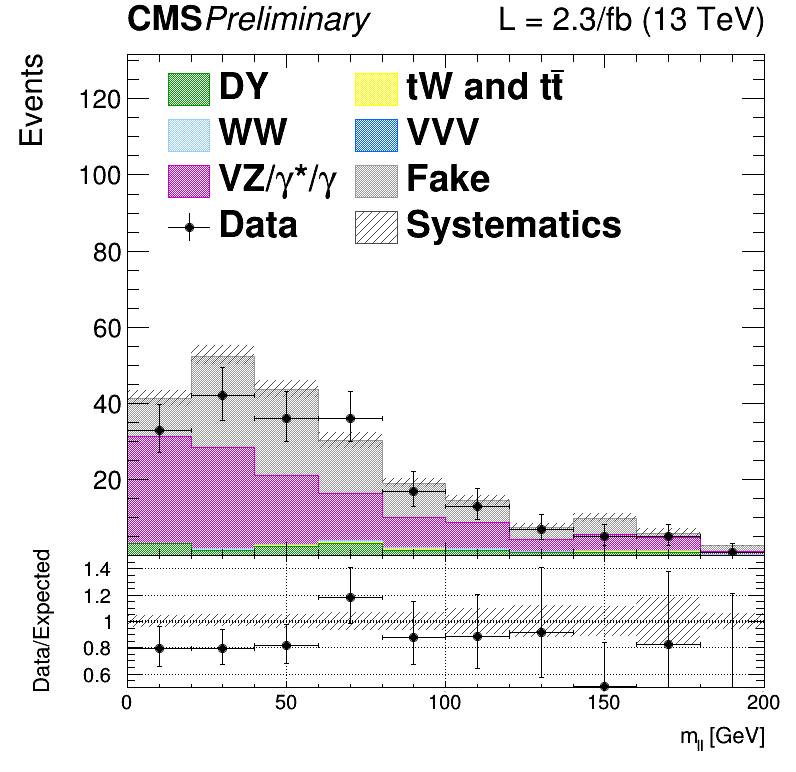
\includegraphics[width=0.45\textwidth]{images/13TeV/cratio_hww2l2v_13TeV_ss_of0j_mll.png}
    }
    \subfigure[1 jet]{
    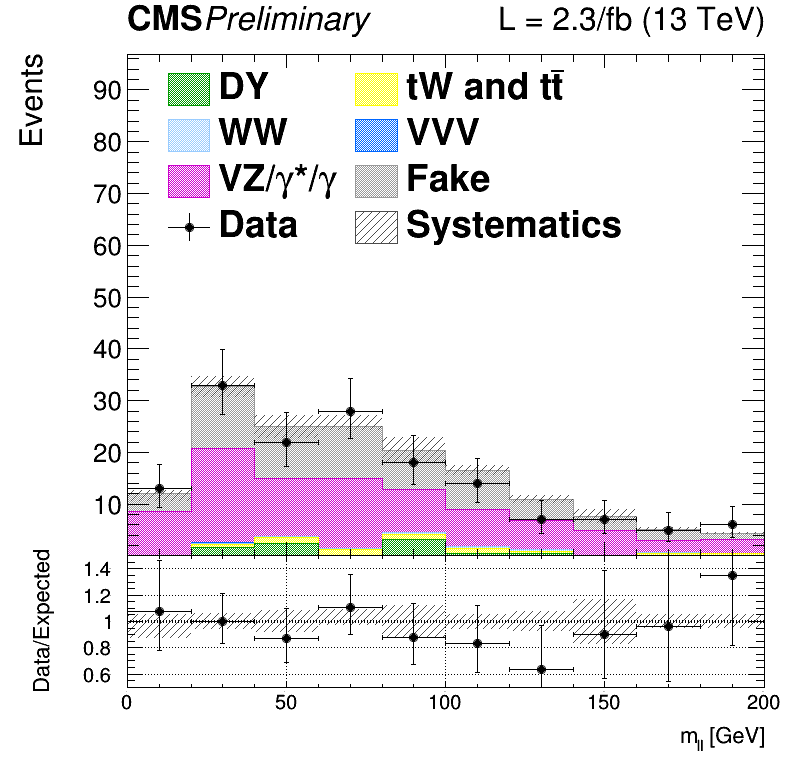
\includegraphics[width=0.45\textwidth]{images/13TeV/cratio_hww2l2v_13TeV_ss_of1j_mll.png}
    }
    \caption{
         Control plots for $m_{\ell\ell}$ in a fakes enriched phase space for events with 0 and 1 jet with $p_{T} > 30$~GeV,
         in e$\mu$ final state.
         Fake contribution has been scaled by 0.8 to match data.
         }\label{fig:13TeVsamesign}
\end{figure}



\subsection{DY background}\label{chap5:DYbackground}

This background contributes to the analysis phase space because of the $\mathrm{Z}/\gamma^*$ decays to a pair of $\tau$ leptons, which consequently decays to an e$\mu$ pair. This background process is predominant in the low \mt region, which is used as an orthogonal control region to determine the background normalization in the 0 and 1 jet categories separately. In particular this control region is defined by selecting events with $\mt < 60$\GeV and $30\GeV < \mll < 80$\GeV. The \mll distributions in these control regions for the 0 and 1 jet categories are shown in Fig.~\ref{fig:13TeVDYtt}.

As for the top quark background, the normalization of this background in the 0 and 1 jet categories, is constrained directly in the fit by means of the control regions, which are treated as two additional categories.

The kinematics of this background is taken from simulation, after reweighting the Z boson \pt spectrum to match the observed distribution measured in data. In fact, this variable is not well reproduced by the MC generator used for simulating this process, especially in the bulk of the distribution, the discrepancy being ascribed to the missing contribution from resummed calculations.

\begin{figure}[htbp]
\centering
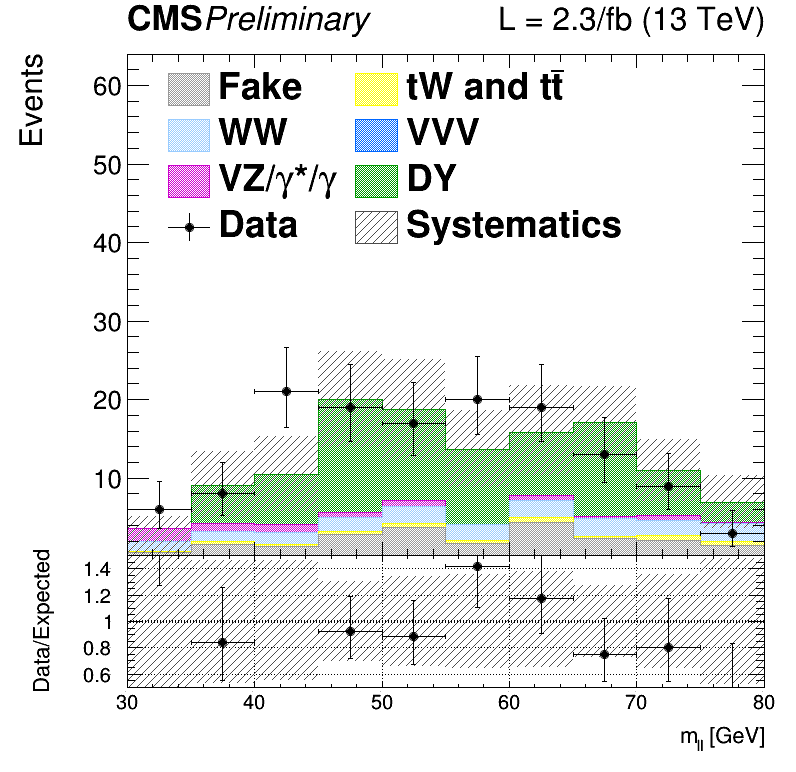
\includegraphics[width=0.45\textwidth]{images/13TeV/cratio_hww2l2v_13TeV_dytt_of0j_mll.png}
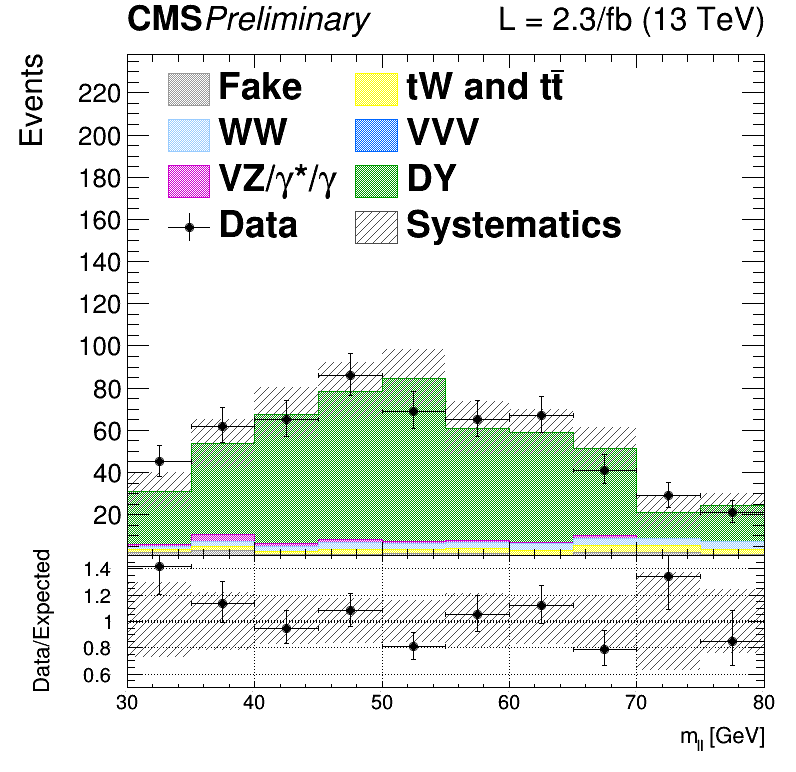
\includegraphics[width=0.45\textwidth]{images/13TeV/cratio_hww2l2v_13TeV_dytt_of1j_mll.png}
\caption{
Distributions of \mll for events with 0 jet (left) and 1 jet (right) in the DY$\rightarrow \tau\tau$  enriched control region. Scale factors estimated from data are applied.
}
\label{fig:13TeVDYtt}
\end{figure}

\subsection{Other backgrounds}\label{chap5:otherBackgrounds}

The W$\gamma^*$ and the WZ electroweak processes can be gathered in the same physical process, although the final state kinematics is rather different. In particular, the invariant mass of the leptons arising from the $\gamma^*$ decays is generally below 4\GeV, while the leptons from the Z boson decay are characterized by a larger invariant mass. Another background which can be experimentally identical to those is the W$\gamma$ production, where a real photon is produced in association with a W boson and consequently undergoes a photon conversion to leptons due to the interaction with the material constituting the first layers of the silicon tracker.

All these backgrounds may contribute to the signal phase space whenever one of the three leptons escape from the detector acceptance or is not identified. The shape and cross section of these backgrounds are taken from simulation. The only exception is the normalization of the W$\gamma^*$ background, being this process dominant in the low \mll region, which is scaled to data defining a proper control region. The control region is defined selecting events with three isolated muons, with $\pt > 10$,5 and 3\GeV for the first three leading muons respectively. The selection is further defined by $\MET < 25\GeV$ and $\MET$ projected to the leading muon $<$ 45\GeV. The pair of muons with the smallest invariant mass is taken as coming from the $\gamma^{*}$ decay. The k-factor measured in data for this background to be applied in the simulation is $1.98\pm0.54$.

All remaining backgrounds from di-boson and tri-boson production, which are of minor importance in the analysis phase space, are normalized according to their expected theoretical cross sections.





